\subsubsection{Fysisk aktivitet og intensitet}\label{subsub:ak_int}
Der er en tydelig sammenhæng mellem puls og kroppens reaktion på den fysiske aktivitet, da den maksimale puls for et individ og intensiteten af den fysiske aktivitet har en lineær sammenhæng. Den maksimale puls kan bestemmes for en person ved at trække personens alder fra en værdi på 220. \citep{CooperBlair2005}\newline
Flere studier påpeger, at procenten af den maksimale puls har sammenhæng med effekten af den fysiske aktivitet. Eksempelvis antallet af forbrændte kalorier, hvorvidt den aerobe udholdenhed trænes, forbedring af den anaerobe tolerance eller forbedring af den kardiovaskulære ydeevne\fxnote{hvilket gør, at man kan sprinte længere / er hurtigere, fordi der kommer mere ilt rundt i kroppen}. I sammenhæng med fysisk aktivitet kræver kroppen adenosintrifosfat (ATP). Dette molekyle er energibærende og nedbrydes løbende for energiudvinding. Anaerobe forhold forekommer, når der ikke er en tilstrækkelig mængde ilt til stede i kroppen, hvorfor denne proces er den første, som indtræder under fysisk aktivitet. ATP kan gendannes anaerobt ved spaltning af kreatinfosfat eller kulhydrater under dannelse af mælkesyre.~\citep{Martini2012,Academic2016c,Engelbreth2010} Under aerobe forhold kan ATP gendannes i store mængder igennem den oxidative fosforylering. Denne proces indtræder og dominerer efter 15-20 minutters fysisk aktivitet. 
\citep{Martini2012,Engelbreth2010} \newline
Pulsen er sigende for aktivitetens intensitetsniveau samt den effekt, som aktiviteten kan medøre for personen. Et højere intensitetsniveau resulterer i en højere puls og dermed hårdere fysisk aktivitet. Denne sammenhæng mellem intensitetszoner, maxpuls, varighed samt fysiologisk udbytte inddeles i fem zoner og ses på \tabref{tab:PA_Procentpuls}. \citep{Leyland2007,Heartratejournal2015}
%\begin{figure}[H]
%	\centering
%	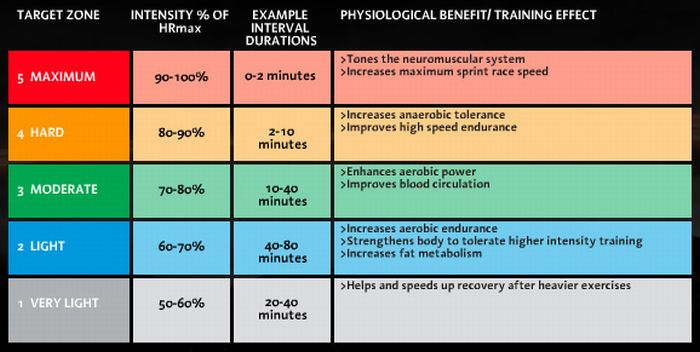
\includegraphics[scale=0.75]{figures/aProblemanalyse/heart-rate-zones.jpg}
%	\caption{På figuren ses fem zoner for kroppens reaktion i forhold til pulsraten. Der ses, at de fem zoner har hver sin påvirkning på kroppen. Det er dog også anbefalet, at varigheden i hver zone bliver lavere desto hårdere aktiviteten er. \citep{Heartratejournal2015}}
%	\label{fig:PA_Procentpuls}
%\end{figure}
\begin{table}[H]
	\centering
	\begin{tabular}{cccc}
		\rowcolor[HTML]{C0C0C0} \hline
		\multicolumn{1}{c}{\cellcolor[HTML]{C0C0C0}Zoner} & \multicolumn{1}{c}{\cellcolor[HTML]{C0C0C0}\begin{tabular}[c]{@{}c@{}}Procent af\\ maksimal puls [\%]\end{tabular}} & \multicolumn{1}{c}{\cellcolor[HTML]{C0C0C0}\begin{tabular}[c]{@{}c@{}}Aktivitetens\\varighed [min]\end{tabular}} & \multicolumn{1}{c}{\cellcolor[HTML]{C0C0C0}Fysiologisk udbytte}    \\ \hline
		\multicolumn{1}{l}{5 - Maksimalt}                & \multicolumn{1}{c}{90-100} & \multicolumn{1}{c}{0-2} & \multicolumn{1}{l}{\begin{tabular}[c]{@{}l@{}}Træner det neuromuskulære system \\og øger maksimal sprinthastighed.\end{tabular}}   \\ \hline
		\multicolumn{1}{l}{4 - Hårdt}                    & \multicolumn{1}{c}{80-90}  & \multicolumn{1}{c}{2-10} & \multicolumn{1}{l}{\begin{tabular}[c]{@{}l@{}}Forbedrer den anaerobe tolerance og\\ øger højhastigheds udholdenhed.\end{tabular}}     \\ \hline
		\multicolumn{1}{l}{3 - Moderat}                 & \multicolumn{1}{c}{70-80}  & \multicolumn{1}{c}{10-40} & \multicolumn{1}{l}{\begin{tabular}[c]{@{}l@{}}Forbedrer aerob styrke og blod-\\cirkulationen.\end{tabular}}      \\ \hline
		\multicolumn{1}{l}{2 - Let}                     & \multicolumn{1}{c}{60-70}  & \multicolumn{1}{c}{40-80} & \multicolumn{1}{l}{\begin{tabular}[c]{@{}l@{}}Forbedrer den aerobe udholdenhed, \\ styrker kroppen til høj intens\\ arbejde og øger fedtmetabolismen.\end{tabular}} \\ \hline
		\multicolumn{1}{l}{1 - Meget let}               & \multicolumn{1}{c}{50-60}  & \multicolumn{1}{c}{20-40} & \multicolumn{1}{l}{\begin{tabular}[c]{@{}l@{}}Hjælper og øger hastigheden af \\ genopbygningen af musklerne efter\\ hård fysisk aktivitet.\end{tabular}} \\ \hline
	\end{tabular}
	\caption{I tabellen ses de fem intensitetszoner, som bestemmes ud fra den maksimale puls. Varigheden for hver intensitetszone angiver tidsintervallet, som aktiviteten skal udføres i for at opnå det tilsigtede fysiologiske udbytte.~\citep{Heartratejournal2015}~(Modificeret)}
	\label{tab:PA_Procentpuls}
\end{table} \vspace{-0.5cm}
Pulsen er en sigende faktor for aktivitetens formål. Dette medfører, at pulsen er bestemmende for intensiteten, varigheden og udbyttet. Intensiteten kan også bestemmes ud fra maksimal iltoptagelse, som er en betegnelse for, hvor meget ilt der optages i minuttet. Derudover kan det bestemmes ud fra Borg skalaen, som er en subjektiv vurdering af, hvor hård en given fysisk aktivitet er. \citep{Kiens2007}